\documentclass[fullpage,twocolumn]{article}

\usepackage{times}
\usepackage{xspace}
\usepackage{cite} % sort citation numbers
\usepackage[breaklinks,colorlinks,
	    linkcolor=blue,citecolor=blue,urlcolor=black]{hyperref}
\usepackage{cleveref}
\usepackage{graphicx}
\usepackage[T1]{fontenc}

%%%%%%%%%%%%%%%%%%%%%%

% Select one or other if want to see comments.
% \com is sometimes displayed during draft.
\long\def\com#1{}
%\long\def\com#1{{\bf \sc comment: }{\small [#1]}{\bf \sc\ endcomment}\newline}

\newcommand{\xxx}[1]{}
%\newcommand{\xxx}[1]{{\color{red} {\bf XXX }{\small [#1]}}}

% Choose regular version or version hacked for arXiv preprint submission
\long\def\arxiv#1#2{#1}			% real version
%\long\def\arxiv#1#2{#2}		% arXiv preprint version

% Choose abbreviated or long-version alternatives in paper
\long\def\abbr#1#2{#1}			% abbreviated version
%\long\def\abbr#1#2{#2}			% long version

% Choose abbreviations or long names/titles in bibliography
%\def\bibbrev#1#2{#1}			% short version
\def\bibbrev#1#2{#2}			% long version
%\def\bibbrev#1#2{\abbr{#1}{#2}}		% follow abbr macro

% Abbreviated or full citation lists: \abcite{basic}{others}
\newcommand{\abcite}[2]{\abbr{\cite{#1}}{\cite{#1,#2}}}

% Conference abbreviations: \bibconf[Nth]{SOSP}{Symposium on ...}
\newcommand{\bibconf}[3][]{#1 \bibbrev{#2}{#3 (#2)}}

% for paralist compactitem envs
%\defaultleftmargin{\parindent}{}{}{}

% Common abbreviations
\newcommand{\ie}{{\em i.e.},\xspace}
\newcommand{\eg}{{\em e.g.},\xspace}

%%%%%%%%%%%%%%%%%%%%%%

\newcommand{\ml}{$\star$ML\xspace}	% The SGML-derived markup languages


\begin{document}

\title{Matchertext: Towards Verbatim Interlanguage Embedding \\
	\Large{\texttt{preliminary draft - not yet for redistribution} \\
	~\\
	Working project repository: \url{https://github.com/dedis/matchertext}}}

\author{Bryan Ford \\ EPFL}

\maketitle

\tableofcontents

\begin{abstract}
Embedding text in one language within text of another is commonplace
for numerous purposes,
but usually requires tedious and error-prone
``escaping'' transformations on the embedded string.
We propose a simple cross-language syntactic discipline,
\emph{matchertext},
which enables the safe embedding a string in any compliant language
into a string in any other language via simple ``copy-and-paste'' --
in particular with no escaping, obfuscation, or expansion of embedded strings.
We apply this syntactic discipline
to several common and frequently-embedded
language syntaxes such as URIs, HTML, and JavaScript,
exploring the benefits, costs, and compatibility issues
in adopting the proposed matchertext discipline.
One early matchertext-based language is MinML,
a concise but general alternative syntax for writing HTML or XML.
\end{abstract}

\section{Introduction}
\label{sec:intro}

The need to embed valid strings in one language into valid strings in another
is commonplace throughout programming practice.
Just a few examples include embedding
regular expressions, URIs, SQL queries, or HTML markup
within string constants in general-purpose programming languages;
JavaScript code embedded in HTML via the \verb|<script>| element;
and URIs embedded as query strings within other URIs,
such as in a query to a service like the
\href{https://archive.org/web/}{Wayback Machine}.

An equally-ubiquitous issue arising from this practice
is the need to transform the embedded string --
generally by \emph{escaping} certain characters sensitive
to the ``host'' language and syntactic context --
so that host language processors will not misinterpret embedded text
as host-language text.
For example,
the regular expression \verb|"[^"]*"| matches double-quoted strings,
but when embedded in a C-like language must be written
like \verb|re.match("\"[^\"]*\"")|,
escaping all the embedded instances of double-quote characters,
so that the embedded quotes will not prematurely end the string literal.
Accidentally forgetting necessary escaping
is naturally a common source of syntax errors in manual embedding practice.
\emph{Automated} embedding is also common practice, however,
such as accepting an arbitrary user-entered string on a web form
and embedding it into HTML via a scripting language like PHP.
With automated embedding,
forgetting to escape embedded strings properly
has become an endless source of critical security bugs
such as SQL injection attacks~\cite{clarke12sql}.

In some future evolution
of today's standard programming languages and practices,
could we achieve the ability to embed any valid string
in essentially any language into any other --
\emph{across languages} --
without ever having to escape, or otherwise transform or obfuscate,
the string to be embedded?
Could we make embedding always a simple matter of verbatim ``copy-and-paste''
when done manually,
or a simple matter of concatenation
or filling a ``hole'' in a tempate
when done automatically?
We propose that the answer can and should be \emph{yes} --
though with important challenges, costs, and caveats of course.

We observe that verbatim interlanguage embedding would be achievable if:
(1)
we could standardize across languages
a set of open/close character pairs
we will call \emph{matchers},
such as the parentheses \verb|()|,
square brackets \verb|[]|,
and curly braces \verb|{}|;
and
(2) 
we could impose the universal ``syntactic discipline''
that \emph{matchers must properly match} in nested pairs
throughout any valid string -- without exception --
in any compliant language.
If \emph{plain text} is an unstructured linear sequence of characters
in a character set like ASCII or Unicode,
then we define \emph{matchertext} to be plain text
conforming to the additional syntactic discipline
that ASCII matchers must match.
For example, the strings `\verb|(a{b}c)|' and `\verb|a({'}["])d|'
are valid matchertext,
while the strings
`\verb|(|', `\verb|{a]|', `\verb|[(])|', and `\verb|}{|'
are plain text but are not valid matchertext.

\begin{figure*}[t]
\begin{center}
\begin{small}
\begin{tabular}{ll}
MRI syntax:	& \verb|http[//search.engine/linksto?site=http[//my.site/]&results=50]| \\
URI syntax:	& \verb|http://search.engine/linksto?site=http%3A%2F%2Fmy.site%2F&results=50| \\
\\
MRI syntax:	& \verb|http[//historical.archive/get?site=http[//my.site/]&year=1998]| \\
URI syntax:	& \verb|http://historical.archive/get?site=http%3A%2F%2Fmy.site%2F&year=1998| \\
\end{tabular}
\end{small}
\end{center}
\caption{Example queries containing embedded resource identifiers
	in URI and MRI syntax for comparison.}
\label{fig:search-query}
\end{figure*}

Consider \emph{matchertext resource identifiers} (MRIs),
a matchertext adapation of
uniform resource identifiers (URIs)~\cite{rfc3986} or
internationalized resource identifiers (IRIs)~\cite{rfc3987}.
A URI like \verb|http://my.site/path/|
may always be transformed to or from
equivalent MRI syntax like \verb|http[//my.site/path]|.
An MRI is embeddable verbatim, with no transformation,
into another MRI or another matchertext-aware language.
Figure~\ref{fig:search-query} shows two example search queries
containing embedded resource identifiers,
contrasting ``copy-and-paste'' embeddable MRI syntax
with traditional URI syntax where the sensitive
colon (\verb|:|) and slash (\verb|/|) characters
must be escaped as \verb|%3A| and \verb|%2F%|, respectively.

\begin{figure*}[t]
\begin{center}
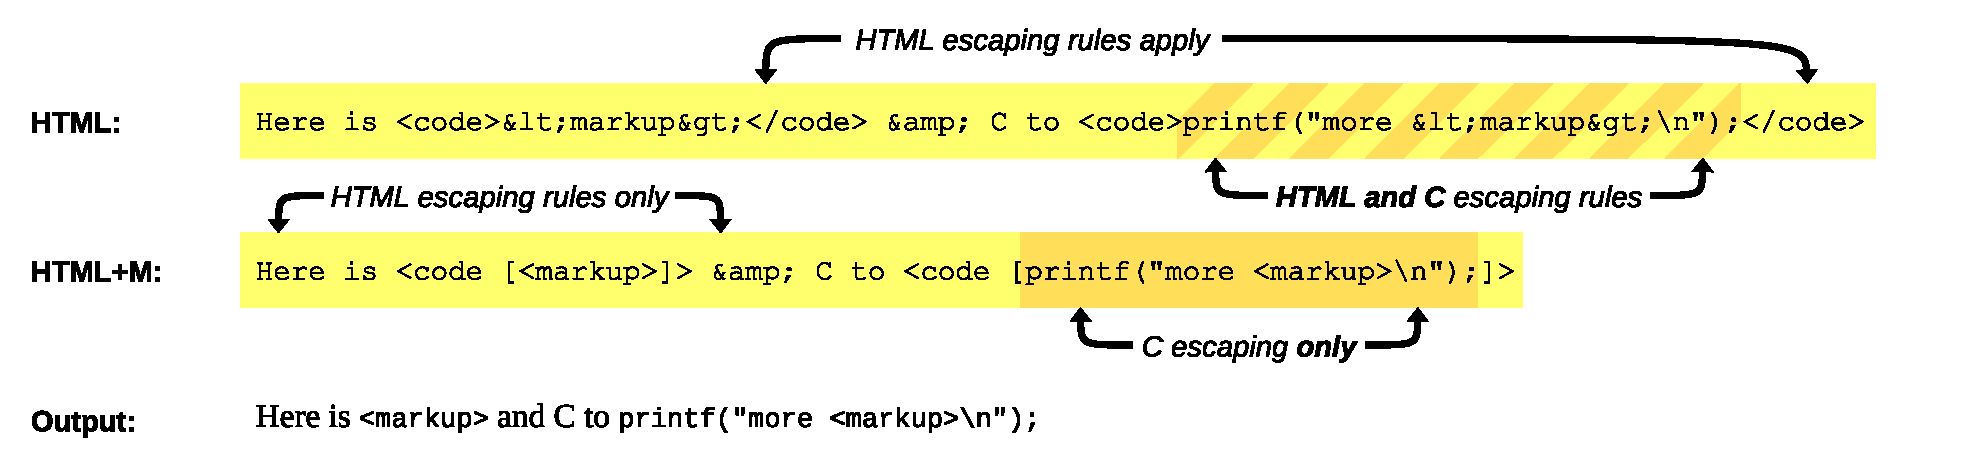
\includegraphics[width=0.95\textwidth]{fig/territorial-integrity.eps}
\end{center}
\caption{Illustration of how different languages' escaping rules
	combine to increase syntactic complexity
	in traditional embedding practice,
	while in matchertext only one language's escaping rules
	are ever active at a given text position.}
\label{fig:territorial-integrity}
\end{figure*}

Adopting the matchertext discipline
does not eliminate the need for character escape sequences:
in fact it can slightly increase the ``escaping obligations''
within a language, as discussed below.
But matchertext enables languages to preserve
the ``territorial integrity'' of their escaping and other syntactic rules,
ensuring that developers need to think about
\emph{only one language's rules at a time}
at any given text position,
even in a string composed from multiple languages.
Thus, matchertext arguably reduces the cognitive load
of writing (or reading) cross-language embedded code.
Figure~\ref{fig:territorial-integrity} illustrates this difference
with a simple example with C code embedded in HTML
including the use of escape codes in both languages.

Existing languages could be adapted incrementally
to support and leverage matchertext.
C-like languages, for example,
might adopt a new escape sequence `\verb|\[|$m$\verb|]|'
to embed an arbitrary matchertext $m$
into a quoted string or character literal.
All characters including quotes and newlines
would be allowed verbatim within $m$,
provided only that matchers match.
Thus,
%\verb|'\[']'| would be equivalent to \verb|'\''|, and
the earlier string-matching regular expression
\verb|"[^"]*"|
could be embedded into a string literal
like \verb|re.match("\["[^"]*"]")|.
We now use an escape sequence
to delimit the entire embedded matchertext,
but we no longer need to add escape sequences
\emph{within} the embedded regular expression.

It is already feasible to write code in existing languages
that is also valid matchertext,
with a bit of care.
Most languages use the matchers in structurally paired forms anyway,
as in expressions like \verb|a*(b+c)|,
lists like \verb|[a,b,c]|,
or maps like \verb|{a:1, b:"hi"}|.
The challenge is mainly in handling the exception cases
where unmatched matchers may commonly appear.

\begin{table*}[t]
\begin{center}
\begin{footnotesize}
\begin{tabular}{ll||ll|ll|ll||ll|ll}
&		& \multicolumn{6}{|l||}{Escapes for C-like languages}
		& \multicolumn{4}{|l}{Escapes for SGML-derived languages} \\
&		& \multicolumn{2}{|l|}{octal escapes}
		& \multicolumn{2}{|l|}{hex escapes}
		& \multicolumn{2}{|l||}{\bf matchers (new)}
		& \multicolumn{2}{|l|}{entity names}
%		& \multicolumn{2}{|l|}{hex}
		& \multicolumn{2}{|l}{\bf matchers (new)}		\\
		&
		& open			& close
		& open			& close
		& open			& close
		& open			& close
		& open			& close		\\
\hline
Parentheses	& \verb|()|
		& \verb|\050|		& \verb|\051|
		& \verb|\x28|		& \verb|\x29|
		& \verb|\o()|		& \verb|\c()|
		& \verb|&lpar;|		& \verb|&rpar;|
%		& \verb|&#x28;|		& \verb|&#x29;|
		& \verb|&o();|		& \verb|&c();|	\\
Square brackets	& \verb|[]|
		& \verb|\133|		& \verb|\135|
		& \verb|\x5B|		& \verb|\x5D|
		& \verb|\o[]|		& \verb|\c[]|
		& \verb|&lbrack;|	& \verb|&rbrack;|
		& \verb|&o[];|		& \verb|&c[];|	\\
		
Curly braces	& \verb|{}|
		& \verb|\173|		& \verb|\175|
		& \verb|\x7B|		& \verb|\x7D|
		& \verb|\o{}|		& \verb|\c{}|
		& \verb|&lbrace;|	& \verb|&rbrace;|
		& \verb|&o{};|		& \verb|&c{};|	\\

\end{tabular}
\end{footnotesize}
\end{center}
\label{tab:unmatched-matchers}
\caption{Potential alternatives in C- and SGML-derived languages
	to escape unmatched matchers in matchertext.}
\end{table*}

One habit we must awkwardly unlearn to write matchertext,
unfortunately,
is using unmatched matchers in quoted strings
to parse or print structured text.
Clauses like \verb|printf("{")| or \verb|case "]"|
are not valid matchertext --
at least not within the string literals.
We must therefore escape these unmatched matchers,
as in \verb|printf("\x7B")| or \verb|case "\x5D"| for example.
Backward-compatible language extensions might ease this pain,
however, 
with new escape sequences that include \emph{both} matchers of a pair
but select only the opener or closer.
The new escape \verb|\o()| represents a literal open parenthesis,
for example,
while \verb|\c[]| represents a close bracket.
Table~\ref{tab:unmatched-matchers} summarizes a few existing and proposed
alternatives for escaping unmatched matchers
in both C-like languages and SGML-derived languages like HTML.

In the rest of this paper, 
we develop more deeply the design and rationale for the matchertext discipline,
then explore how a number of common languages of varying types
might be incrementally adapted to support and leverage
the matchertext discipline effectively.

This work is in an early exploration and experimentation phase,
so the evaluation is currently a placeholder,
serving as a preliminary map for the ways in which
we \emph{would like to} evaluate matchertext
and its use in practical languages.
Some key questions we would like to answer include:
how common (and how painful) is the need for escaping
in the most common cross-language embedding scenarios?
How extensively would large existing repositories of code or data
need to be modified in order to convert them to matchertext?
How does matchertext affect the usability to users or developers
of common constructs in common embedding use-cases,
such as synthesizing or editing HTTP or SQL queries?
How does matchertext affect the frequency of syntax-related bugs --
especially those potentially leading to security vulnerabilities --
in code from typical developers?


\xxx{
Caveats:
- does not eliminate other needs for escaping (just escaping for embedding).
- does not eliminate the need for correct input validation
in automated embedding
(e.g., checking that the input is matchertext
or transforming it into matchertext)),
and thus cannot be expected to eliminate all syntax-related security bugs
of the SQL injection variety.
Mistakes will still happen.
However, we may hope that the consistent and rigorous application
of the matchertext discipline
might significantly increase the robustness of embedding practices
and hence decrease the frequency of such bugs.
XXX to be tested empirically.
}

\xxx{ paper roadmap}


\subsection*{An open research project}

This draft represents a ``work-in-progress'' snapshot
of an experimental open research project.
Anyone with adequate interest, skills, and motivation
is welcome to contribute to this research project,
and potentially become a co-author upon making a substantial contribution.
(Smaller contributions will receive acknowledgments in the final paper.)
To propose a contribution, please use Pull Requests (PRs)
on the project's GitHub repository.
We do not have time and cannot promise to answer all E-mails,
or provide detailed guidance,
before an interested potential contributor has proactively
created and submitted some significant and well-considered contribution.


\section{Background: needs and pitfalls of interlanguage embedding}
\label{sec:bg}

\subsection{Needs for embedding}

special-purpose ``little languages'' that are usually embedded.
URIs. regexps. JSON. SQL.

Shells, scripts, and command-line escaping.
Log files.

Larger languages.  JavaScriopt/TypeScript within HTML/XHTML.
Template-driven authoring languages (e.g., Hugo).

\xxx{ explore: PHP-generated HTML with inline JavaScript.
See for example \href{http://www.zedwood.com/article/how-to-properly-escape-inline-javascript}{How to properly escape inline javascript} }

\href{https://en.wikipedia.org/wiki/Leaning_toothpick_syndrome}{"leaning toothpick syndrome"}

\subsection{What often goes wrong}

Convenience challenges.

Error-proneness issues.

Destructive interaction of inner and outer escaping mechanisms.

Multiple levels of embedding: exploding complexity of manual escaping;
potentially-exponential expansions with automatic escaping.
(e.g., C-like escaping: `\verb|\|' becomes `\verb|\\|'
and `\verb|"|' becomes `\verb|\"|',
so $2^l$ size with $l$ levels of escaping.)


Long quotes.  
triple-quotatins might indeed be less likely to appear
in a big text cut-and-pasted into a file,
but it still \emph{may} unexpectely appear.
The same goes with long-inclusion ...

\subsection{When security goes wrong}

armoring of untrusted inputs,
and what happens when that isn't done [correctly].

TODO: Review the security literature for this kind of security bug.


\section{Matchertext design and rationale}
\label{sec:design}

\subsection{Abstract matchertext}

basic principle, given some set of matcher pairs --
but leaving the decision of which pairs for later in
\cref{sec:design:ascii}

Basic rule: in matchertext, \emph{matchers must match}.

Always-embeddability given that embedded string is valid matchertext.

We assume some alphabet $A$.
We further assuma a set $M$ of $k$ matcher pairs
$\{(o_1,c_1),\dots,(o_k,c_k)\}$,
where $o_1,\dots,o_k$ are \emph{openers} in $A$,
and $c_1,\dots,c_k$ are corresponding \emph{closers} in $A$.
Let the set $N$ of \emph{nonmatchers} be the subset of $A$
excluding openers and closers:
\ie $N = A \setminus \{o_1,\dots,o_n,c_1,\dots,c_n\}$.
A \emph{nonmatcher string} $n$ is a string of any finite length
(including empty)
consisting only of nonmatchers in $N$.

\xxx{Epsilon for alphabet, tradition.}

We can inductively define the language $L$ of \emph{matchertext strings}
as follows:
\begin{itemize}
\item	For any nonmatcher string $n$,
	$n$ is a matchertext string.
\item	For any matchertext string $m$,
	any corresponding open/close pair $(o_i,c_i) \in M$,
	and any nonmatcher strings $n_1$ and $n_2$,
	the concatenation $n_1\,o_i\,m\,c_i\,n_2$ is a matchertext string.
\end{itemize}

By construction, every opener is always paired
with the corresponding closer later in the string,
while nonmatchers may be interspersed without restriction.

By the above definition,
matchertext fulfills the classic definition of a syntactic \emph{language} --
namely a set of strings mathematically defined to be in the language.
In practice, however,
we will refer to matchertext as a \emph{syntactic discipline}
rather than a language
because matchertext is devoid of semantic meaning,
or even any syntactic structure outside the rule that ``matchers must match.''
Matchertext is intended only to provide a structural background rule
atop which any number of \emph{matchertext languages} may be defined,
each with its own syntax further constraining the set of valid strings,
and perhaps associating language-dependent semantic meaning to those strings.
In particular, we can in principle take any arbitrary language $L$
defined as a set of strings,
and define the \emph{matchertext subset} of $L$
simply as those strings $s \in L$ that are also matchertext strings.



\subsubsection{Character set and encoding}

The matchertext discipline does not dictate any particular choice
of character set or encoding.
For example, a matchertext string or text file could be in plain ASCII,
in Unicode/UCS encoded via UTF-8 or UTF-16,
in any of the numerous pre-Unicode character sets and encodings,
or in any subset of one of these character sets.
The matchertext rule merely states that
wherever the ASCII matchers
\verb|()[]{}|
%\verb|(|,\verb|)|,\verb|[|,\verb|]|,\verb|{|,\verb|}|
might appear in plain text,
they must occur in matched pairs.
A plain text string in a character set restricted to contain no ASCII matchers
is trivially matchertext,
because it by definition has no characters
that could violate the matchertext rule.

One implication of this orthogonality between the matchertext rule
and character set choice
is that residual syntactic issues may still arise
whenever a host language might ``disagree'' with an embedded language
on character set choices.
Matchertext addresses some embedding issues, but not all of them.
We will return to this issue later in \cref{sec:embed:mri:liberal}
when we consider character set constraints
in uniform resource identifiers (URIs).


\subsection{Embedding considerations}

If a host language $L_H$ wishes to embed a language $L_E$,
then in the contexts where strings of $L_E$ are expected,
$L_H$ must impose \emph{no} constraints on characters allowed
other than the matchertext discipline (matchers must match).
Further $L_H$ must not transform the embedded strings of $L_E$ in any way
while extracting and interpreting the embedded string.
Specifically, any escaping mechanisms or other transformations
that might normally apply to text in $L_H$
must be disabled in the context of the embedded string.
If any escaping mechanisms or other transformations
are active within the embedded string,
those must be that of $L_E$, not $L_H$.

\xxx{Example with MRIs?}

\xxx{Formalization?}


\subsection{Why must the matchers be standardized?}



\subsection{Why ASCII matchers?}
\label{sec:design:ascii}

Why the ASCII matchers?
To achieve interlanguage embeddability,
we must agree on a cross-language standard for what character pairs
pairs the sensitive matchers are.
There is a strong tradition among most text-based machine-readable languages
to use the ASCII punctuation characters -- and mostly \emph{only} those --
as sensitive characters delimiting structural concepts
and denoting hierarchical relationships.
In particular, the three ASCII matcher pairs --
the parentheses `\verb|(|',`\verb|)|',
the square brackets `\verb|[|',`\verb|]|',
and the curly braces `\verb|{|',`\verb|}|' --
are almost always used in matched pairs
(if used for syntactically-sensitive purposes at all)
in most programming languages and other machine-readable syntaxes.


Why all the ASCII matchers?  More redundancy, more robustness
to undetected accidental errors or bugs.

Why not the ASCII angle brackets?

Why not the Unicode matchers too?


\subsection{Writing matchertext in existing languages}

In most popular langguages whose input is normally plaintext,
it is already \emph{possible} -- using existing escaping mechanisms --
to write a matchertext version
(either manually or automatically)
that is at least semantically equivalent
to any given valid plaintext string in that language.

Consider URIs, for example,
which have a standard percent-escape code mechanism
to replace potentially-sensitive ASCII characters with hexadecimal escape codes.
By RFC XXX, URIs are normally not supposed to contain square brackets anyway
except in matched pairs as part of IPv6 address syntax.
But URIs may contain parentheses and curly braces (XXX ?),
which might be unmatched in an arbitrary URI.
Such an URI can always be rewritten
into a semantically-equivalent matchertext URI
(i.e., one that evaluates to the same canonical form XXX)
by replacing all unmatched matcher characters with their
equivalent percent-escape codes.
For example, the URI `\verb|scheme://site/open(|'
would become `\verb|scheme://site/open%28|',
`\verb|scheme://site/close)|'
becomes `\verb|scheme://site/close%29|'
and `\verb|scheme://site/close)open(|' becomes
`\verb|scheme://site/close%29open%28|'.
The URI `\verb|scheme://site/open(close)|'
need not be rewritten at all,
since all the matchers it contains already (happen to) match.

In SGML-derived languages such as HTML and XML, similarly,
any valid plaintext string in the language
can generally be converted to an equivalent matchertext string
simply by replacing all unmatched ASCII matchers
with the decimal escape codes
`\verb|&#40;|', `\verb|&#41;|' or
`\verb|&lpar;|', `\verb|&rpar;|' for parentheses,
`\verb|&#91;|', `\verb|&#93;|' or
`\verb|&lbrack;|', `\verb|&rbrack;|' for square brackets, and
`\verb|&#123;|', `\verb|&#125;|' or
`\verb|&lbrace;|', \verb|&rbrace;|' for curly braces.

This does not mean that rewriting unmatched matchers into moderately-obscure
(especially numeric) escape codes
is particularly convenient or enjoyable to do manually, of course.
Fortunately, given the prevalence with which ASCII matchers
tend to be used in properly-matched fashion anyway --
both in programming languages and in free-form human-language text strings --
there is at least hope that we need not worry about escaping unmatched matchers
\emph{all the time}.
(XXX we will explore this question of frequency in the evaluation.)
But \emph{sometimes} we will still need to express
unmatched matcher characters in many languages --
when we are trying to ``talk about'' those matchers
as \emph{literal characters}, for example,
whether in code or human-readable text.

\subsection{Matchers in character and string literals}

It is near-ubiquitous practice in mainstream programming languages 
to use the ASCII single- and/or double-quote characters (\verb|'|, \verb|"|)
to delimit literal characters or strings.

\subsection{Gracefully evolving towards matchertext-friendly languages}

We can envison backwards-compatible extensions to most popular languages
that could 


\subsection{Unmatched matchers in comments}



\section{Host language considerations}
\label{sec:host}

...

One important observation is that
languages need not \emph{be} matchertext-compliant in their syntax
just in order to \emph{host} embedded matchertext.
Host languages can preserve full compatibility
with all their existing (non-embedded) code --
continuing to allow unmatched matchers in string constants for example --
while incrementally adding extensions that make it easy
to embed matchertext strings verbatim within the host language.


\subsection{C-like host languages}


\subsection{SGML-style markup host languages}

While the venerable
Standard General Markup Languages (SGML)~\cite{iso8879sgml}
itself has waned in popularity,
its derivatives HTML~\cite{whatwg22html} and XML~\cite{w3c08xml}
are now ubuiquitous in Web content and programming.
Wherever the differences between these markup languages do not matter,
we will refer to them all as \ml languages.

In their basic role as markup languages
used to produce rich, structured documents,
\ml languages frequently play ``host'' to embedded strings
in countless other languages:
typically, in the language(s) of software or APIs
that a marked-up document is written about.
Embedding code in other languages as verbatim text
is a basic and frequently-used purpose of HTML's
\verb|<code>| and \verb|<pre>| tags,
for example.
Beyond merely marking up verbatim text in other languages, however,
HTML in particular has evolved to include special-purpose support
for embedding several other languages within HTML:
namely scripting languages such as JavaScript or Tcl,
cascading style sheets (CSS)~\cite{XXX},
MathML~\cite{XXX},
and SVG~\cite{XXX}.

The \ml languages are surprisingly complex syntactically,
especially given their simple-sounding purpose
of ``merely'' describing structured markup of usually human-readable text.
In particular,
there are at least three different syntactic contexts
in which strings in other languages are often embedded
into \ml languages --
and in which three different sets of quoting and escaping rules apply.
Embedded strings are often embedded
(1) as the content of an element,
(2) as an attribute within an element's start tag, or
(3) as verbatim text within a CDATA section.
We address each of these syntactic contexts in turn,
in each case suggesting potential matchertext extensions
that could help mitigate the various forms of ``escaping hell''
that these embedding contexts can create.

\begin{figure*}
\begin{center}
\begin{footnotesize}
\begin{tabular}{lrl}
\multicolumn{3}{l}{\textbf{(a) Embedding strings in other languages as element content, in standard HTML or with matchertext hosting extensions (+M):}} \\
& HTML	& \verb|<code>printf("Hello world!");/code>| \\
& +M	& \verb|<code [printf("Hello world!");]>| \\
& HTML	& \verb|<code>printf("Example &lt;b&gt;bold&lt;/b&gt; and &amp;bigstar; character in HTML");]>| \\
& +M	& \verb|<code [printf("Example <b>bold</b> and &bigstar; character in HTML");]>| \\
& HTML	& \verb|<script>document.getElementById("demo").innerHTML = "Hello world!";</script>| \\
& +M	& \verb|<script [document.getElementById("demo").innerHTML = "Hello world!";]>| \\
& HTML	& \verb|<script>document.getElementById("demo").innerHTML = "a <" + "/script> end tag";]>| \\
& +M	& \verb|<script [document.getElementById("demo").innerHTML = "a </script> end tag";]>| \\
\\
\multicolumn{3}{l}{\textbf{(b) Embedding strings in other languages within element attributes:}} \\
& HTML	& \verb|<button onclick="okClicked()">OK</button>| \\
& +M	& \verb|<button onclick=[okClicked()]>OK</button>| \\
& HTML	& \verb|<button onclick="emitCharacter('\'')">Emit Apostrophe</button>| \\
& +M	& \verb|<button onclick=[emitCharacter("'")]>Emit Apostrophe</button>| \\
\\
\multicolumn{3}{l}{\textbf{(b) Embedding strings in other languages within CDATA (character data) sections:}} \\
& HTML	& \verb|<code>example <![CDATA[<b>bold</b>]]> markup</code>| \\
& +M	& \verb|<code>example <![MDATA[<b>bold</b>]]> markup</code>| \\
& HTML	& \verb|<code>example <![CDATA[<![CDATA[character data]]]]><![CDATA[>]]> markup</code>| \\
& +M	& \verb|<code>example <![MDATA[<![CDATA[character data]]>]]> markup</code>| \\
& HTML	& \verb|<code>example <![CDATA[<![CDATA[<![CDATA[double embedded]]]]]]>| \\
&	& \verb|<![CDATA[><![CDATA[>]]]]><![CDATA[>]]> markup</code>| \\
& +M	& \verb|<code>example <![MDATA[<![MDATA[<![MDATA[double embedded]]>]]>]]> markup</code>| \\
\end{tabular}
\end{footnotesize}
\end{center}
\label{fig:ml-emb}
\caption{Examples of embedded strings in standard HTML
	and with potential matchertext extensions (+M).}
\end{figure*}


\subsubsection{Strings embedded as element content}

One common form of embedding into \ml 
is marked-up text serving as the content of an element:
\eg example code between \verb|<code>| and \verb|</code>| tags
or between \verb|<pre>| and \verb|</pre>| tags in HTML.
Further, the \verb|<script>| and \verb|<style>| tags in HTML
exist specifically to embed scripting language code
and cascading style sheet (CSS) code, respectively,
as their content.

The syntactic rules governing
what can appear in text embedded as element content,
however,
depend intricately on the tag, the d\ml language in question,
and even the language version.
In most elements such as \verb|<code>| and \verb|<pre>|,
any characters \verb|<| and \verb|&| appearing in the embedded string
must be escaped (as \verb|&lt;| and \verb|&amp;|),
to prevent the \ml parser misinterpreting them as
the start of a tag or a character reference,
respectively.
In XML, this rule applies to the content of all element,
including the content of \verb|<script>| and \verb|<style>| tags
of XML-based XHTML.
In HTML, however, the content of \verb|<script>| and \verb|<style>| tags
is raw character data,
uninterpreted by the HTML parser except to find the end tag.
The content of such tags therefore \emph{can} contain
unescaped \verb|<| and \verb|&| characters --
and \emph{cannot} use HTML character entity references for escaping.
In HTML4, this uninterpreted content is terminated
by the first instance of a \verb|</| character sequence,
whether or it is part of the corresponding end tag
(\verb|</script>| or \verb|</style>|).
HTML5 in contrast terminates the content with a sequence \verb|</|
followed by the appropriate end tag name.
In all of these cases, figuring out what \emph{must be},
what \emph{can be}, and what \emph{cannot be}
escaped is subtle and potentially confusing.

As a potential extension enabling any of the \ml languages
to host embedded matchertext conveniently,
we suggest the following new element syntax:

\begin{center}
\verb|<|\emph{name attributes }\verb|[|\emph{matchertext content}\verb|]>|
\end{center}

The \emph{name} and \emph{attributes} are the tag name and optional attributes
as they normally appear in a start tag,
and \emph{matchertext content} is the element content as literal matchertext
enclosed in square brackets,
uninterpreted except to find the end by matching matchers.
This syntax represents the entire element,
with no end tag,
so it is more concise than traditional start/end tag pairs.
Since the content within brackets is uninterpreted except to match matchers,
the content cannot contain further markup (child elements)
or \ml character entity references when using this syntax.

\Cref{fig:ml-emb}(a) illustrates a few examples
of embedding JavaScript into a \verb|<code>| or \verb|<script>| element,
either in standard HTML or with the proposed matchertext content syntax (+M).
The first example is for embedding trivial and non-problematic code.
The second example illustrates the more troublesome corner case
where the embedded JavaScript wishes to output
an \verb|</script>| end tag within a string literal.
Since HTML entity references are unavailable within a \verb|<script>| element,
the code must either use JavaScript escapes,
or construct the \verb|</script>| tag from two string literals,
to prevent the embedded string literal from prematurely ending
the \verb|<script>| element.
In matchertext content syntax,
neither example is problematic and both are more concise.


In XML, which is much more strict than HTML,
the `\verb|<|' and `\verb|>|' characters (which delimit tags)
and `\verb|&|' characters (which introduce entity references)
are not allowed at all in element content,
and hence must normally be escaped as
\verb|&lt;|, \verb|&gt;|, or \verb|&amp;| respectively.
Similarly, single quotes \verb|'| must be escaped as \verb|&apos;|
in single-quoted attribute values,
and double quotes \verb|"| must be escaped as \verb|&quot;|
in double-quoted attribute values.

\xxx{ explore: PHP-generated HTML with inline JavaScript.
See for example \href{http://www.zedwood.com/article/how-to-properly-escape-inline-javascript}{How to properly escape inline javascript} }


\subsubsection{Strings embedded as attribute values}

Besides element content,
scripting language code is often embedded in the attribute values
of \ml start tags,
most commonly to handle events in active user interface elements.
Attribute values represent a different syntactic context
in which different escaping rules apply.
When attribute values are delimited with single or double quotes,
the quote character that introduced the value must be escaped
(as \verb|&apos;| or \verb|quot;|)
if it is embedded in the attribute value.
Character references may appear and are substituted in attribute values,
like normal elements such as \verb|<code>| in HTML
but unlike \verb|<script>| or \verb|<style>| content.
As \href{https://www.w3.org/TR/html401/appendix/notes.html#notes-specifying-data}{the HTML specification notes},
this means that script and style data cannot be simply
cut-and-pasted between element content and attribute values
without care for the changed escaping rules.
HTML forgivingly allows \verb|<| and ``unambiguous'' \verb|&| characters
to appear unescaped in attribute values,
while XML requires them to be escaped (along with the active quote character).

One potential matchertext hosting extension
would be simply to allow square brackets as a third ``quoting style''
for attribute values,
where the text between the brackets is uninterpreted
except to match matchers and find the end.
With this extension as well as the above,
the quoting and escaping environments for matchertext element content
and matchertext attribute values would be identical,
allowing code to be cut-and-pasted between these contexts freely.

\Cref{fig:ml-emb}(b) illustrates examples
of script text embedded in attribute values,
without and with matchertext hosting extensions.
The second illustrates the fact that any time
a character or string literal is needed in such embedded text,
the embedding effectively ``consumes'' both quote characters
in standard HTML or XHTML,
while matchertext embedding preserves JavaScript's ``syntactic freedom''
of using one quote character to quote a verbatim instance of the other.


\subsubsection{Strings embedded in CDATA sections}

A third syntactic context in which strings are often embedded in \ml
is via CDATA sections of the form \verb|<![CDATA[|\emph{text}\verb|]]>|,
where \emph{text} is mostly-uninterpreted character data.
Note that CDATA \emph{sections} are distinct from
CDATA-typed \emph{entities} or \emph{attributes}
as declared in an SGML document type definition (DTD).
CDATA sections offer the ``greatest protection''
from typical \ml escaping requirements,
in that \emph{only} the section-terminator sequence \verb|]]>|
is disallowed within the embedded text.
Because \ml escape sequences are unavailable within CDATA sections, however,
they also require the most-awkward syntactic contortions
in the hopefully-rare event that a \verb|]]>| sequence
needs to appear in an embedded string.
This ``worst-case scenario'' readily comes to pass
whenever one is \emph{writing about} CDATA sections and their issues
in a \ml markup language, for example.

A straightforward extension to host matchertext in a CDATA-like section
would be simply to add a matchertext section form
such as \verb|<![MDATA[|\emph{matchertext}\verb|]]>|,
where \emph{matchertext} is uninterpreted matchertext.
\Cref{fig:ml-emb}(b) illustrates three examples of markup
using CDATA sections versus corresponding MDATA sections.
The first example is simple and non-problematic in either case.
The second example illustrates how MDATA sections eliminate the problem
of embedding a \verb|]]>| sequence within such a verbatim section --
provided that matchers still match, of course.
The third example shows the more-extreme case of ``double embedding'' --
where the complexity and visual obfuscation of CDATA sections explodes,
while MDATA sections nest arbitrarily with no difficulty.
This double-embedding scenario might seem contrived,
but it is exactly what is needed, for example,
when attempting to write in \ml markup a visual example
(\eg in a \verb|<code>| block)
of the single-embedding problem and its standarde ``preferred'' solution
of replacing \verb|]]>| sequences with \verb|]]]]><![CDATA[>| sequences
to ``close and reopen'' the outer CDATA section.



\section{Embedded syntax considerations}
\label{sec:embed}

Having focused above on host language considerations,
we now switch focus to considerations for languages
to \emph{be embedded} as matchertext.
The languages of interest for embedding
overlaps heavily with those of interest as host languages;
we separate these discussions mainly to emphasize the orthogonality
of host- and embedded-language issues and cleanly separate them.

It is already readily feasible to write valid matchertext
in most of the languages we will consider for embedding.
This is because most popular machine-readable languages
already largely conform to the ``matchers must match'' rule
in their explicit uses of the matcher characters.
Violations of the matchertext rule most commonly occur
only in embedded ``free-form'' text such as string literals and comments.
The language extensions we will propose are motivated almost exclusively
by increasing convenience and visual clarity,
and are by no means essential.

\subsection{String literals in C-like languages}
\label{sec:embed:c}

Almost certainly the most common context in which unmatched matchers
appear in most today's existing source code is within string literals.
This is especially true of code to print, or parse,
machine-readable code in almost any syntax.
Structured pretty-printing code frequently includes code sequences like this:

\begin{quote}
\verb|print("[")| \\
\emph{output all elements of a list} \\
\verb|print("]")|
\end{quote}

Similarly, parsing code often uses \verb|if|, \verb|switch|,
or \verb|case| conditionals
to recognize and parse matcher-delimited syntactic structures,
as in:

\begin{quote}
\verb|if peekNextChar() == '[':| \\
\verb|  scanChar('[')| \\
\verb|  |\emph{scan all elements of a list} \\
\verb|  scanChar(']')| 
\end{quote}

Printing and scanning code like this generally violates the matchertext rule,
and adapting such code most likely represents the biggest ``pain point''
in any venture to write readily-embeddable matchertext.

Almost all programming languages already offer a workable
if slightly cumbersome solution:
simply replace unmatched matchers in string literals
with suitable numeric character escapes.
Instead of \verb|print("[")|, for example,
write \verb|print("\x5B")| (C, C++, JavaScript)
or \verb|print("\u005B")| (Java, JavaScript, Go).
This always works;
the main annoyance is that it requires the writer (and reader) of the code
to remember or look up the codes for the matcher characters in an ASCII table.

The usual solution in C-like languages
to handle ``special'' characters in string literals
is simply to backslash-escape the special character,
like \verb|\[|.
This traditional solution does not work for unmatched matchers in matchertext,
however,
because the matchertext rule is deliberately language-independent
and oblivious to language-specific syntax such as that of string literals.
So a backslash-escaped unmatched bracket \verb|\[|
remains just as much a matchertext violation as the bracket alone.

There is a solution that avoids the need for ASCII tables, however.
Because literal matchers are a problem in matchertext only when unmatched,
we can simply introduce escape sequences that incorporate
\emph{both} matchers as a properly-matched pair,
while ``selecting'' only the opener or closer of the pair.
In C-like languages, for example,
we suggest the sequence \verb|\o()| to escape an open parenthesis,
\verb|\c()| to escape a close parenthesis.
Similarly,
\verb|\o[]| and \verb|\c[]| represent open/close square brackets,
and \verb|\o{}| and \verb|\c{}| represent open/close curly braces.

The choice of the letters \verb|o| and \verb|c| to escape the matchers
is consistent with their standardized character classes:
\href{https://www.compart.com/en/unicode/category/Ps}{``Open Puntuation (Ps)''}
and
\href{https://www.compart.com/en/unicode/category/Pe}{``Close Punctuation (Pe)''},
respectively.
We might consider \verb|l| and \verb|r| for ``left'' and ``right'',
escept \verb|\r| is a near-universal escape for carriage return (CR).
A few languages already use \verb|o| or \verb|c| in escape sequences:
\eg Raku uses \verb|\o[|$n$\verb|]|
to denote the ASCII character with octal value $n$,
and uses \verb|\c[|$n$\verb|]|
to denote a Unicode character with name or decimal value $n$.
Many of these existing uses are technically not in conflict syntactically,
provided the existing use requires a non-empty string between the matchers --
as Raku does in the above cases, for example.
% see raku/escapes.raku for a trivial script with which to verify this.
In any case, different languages need not agree
on specific escapes sequences for unmatched matchers
and are free to make their own stylistic choices.


\xxx{relationship: triple-quoted/multiline literals}


\subsection{Comments and derived documentation}

Another context in which unmatched matchers may regularly appear
in typical source code is within comments:
\eg as part of human-readable text \emph{describing}
how the associated code handles particular characters.
Conventional language processors usually just ignore unmatched matchers
(along with everything else) in a comment.
But the matchertext discipline operates below and oblivious to
the syntax of a particular language,
and hence does not know what a ``comment'' is --
so the matchertext discipline must disallow unmatched matchers even in comments.

Since comments are generally intended for humans reading the source code,
it is usually possible simply to rephrase the comment
to avoid a literal use of unmatched matcher characters:
\eg just name it (`open parenthesis')
instead of writing it (`\verb|(|').
Another alternative,
if a language adopts the above extensions for string literals,
is simply to use these matchertext-friendly escapes in comments as well
(\eg \verb|\o()|).

In some languages,
comments often get used to produce API documentation,
using tools like \href{https://www.oracle.com/java/technologies/javase/javadoc-tool.html}{Javadoc}
or \href{https://pkg.go.dev/golang.org/x/tools/cmd/godoc}{godoc}.
In such cases,
it may be useful to interpret escape sequences such as those above
while auto-generating documentation from source code,
so that a documentation comment like `\verb|// Parse a \o()|'
becomes `Parse a (' in the formatted output generated from the code.


\subsection{SGML-derived languages}
\label{sec:embed:ml}

Considerations similar to those above for string literals
apply when we wish to embed \ml-language markup
into other languages as matchertext.
The most common reason unmatched matchers appear in markup
is when needed in literal text being marked up:
\eg human-readable text \emph{about} the matcher characters
or syntactic constructs built from them,
or code examples that contain unmatched matchers.

As with C-style string literals,
\ml languages already offer a workaround:
simply use character references,
either named (like \verb|&lpar;|)
or numeric (\verb|&#x0028;|).
For the same reasons as above,
we may like to have extensions
offering more visually-obvious alternatives for writing matchertext:
\eg \verb|&o();| and \verb|&c();|
for open and close parentheses, 
respectively.


\subsection{Uniform resource identifiers}
\label{sec:embed:uri}

Since uniform resource identifier (URI) syntax represents
a special-purpose ``little language'' just for expressing identifiers,
URIs are predominately embedded in other contexts --
software source code, documentation markup, configuration files, etc.
Especially since URIs are intended to be human-readable,
it would thus seems useful if URIs
could be maximally ``friendly'' for embedding.

\subsubsection{The near-matchertext-compliance of URIs}

Conventional URI syntax~\cite{rfc3986}
already ``nearly'' complies with the ``matchers must match'' rule
and is thus, usually, embeddable verbatim in a matchertext context.
Curly braces are formally disallowed in URIs.
Square brackets are allowed \emph{only} to surround IPv6 addresses
in the authority field,
in properly-matched fashion.
Thus, the only unmatched matchers that \emph{can} exist
in a strictly-valid URI are parentheses.
Even these, when appearing in URIs,
often still come in matched pairs anyway.\footnote{\begin{tiny}
	For example:
	\texttt{https://en.wikipedia.org/wiki/URI\_(disambiguation)}
	\end{tiny}}

In the rare cases when unmatched parentheses are ``needed'' in a URI,
they may always be percent-escaped as \verb|%28| or \verb|%29|.
For example, the string `\verb|open(|'
becomes `\verb|open%28|' in a matchertext URI,
`\verb|close)|'
becomes `\verb|close%29|',
and `\verb|close)open(|' becomes
`\verb|close%29open%28|'.
The string `\verb|open(close)|'
need not be rewritten at all in a matchertext URI,
since the matchers it contains already happen to match.

We could always consider escaping extensions
such as \verb|%o()| and \verb|%c()|,
but it is far from clear that their likely-marginal need
would justify the syntactic complexity in this case.
Even if URI syntax is liberalized further to allow
square brackets and/or curly braces in components,
it is unclear how commonly unmatched matchers would be needed,
since it is not particularly common to write parsing or scanning code
within a URI for example.


\subsubsection{The URI end-finding problem}
\label{sec:embed:uri:end}

Nevertheless, 
URI syntax does suffer from at least one significant usability flaw
arising from its frequent use as an embedded syntax.
URIs can and often do appear almost ``anywhere''
in freeform human-readable text --
\eg typed or copied into E-mails, notes, documents, etc.
Smart text editors often try to detect URIs on entry
and automatically turn them into hyperlinks --
but these heuristics can easily break because
there is no unambiguous syntactic separation between the URI
from surrounding (particularly following) text.
Suppose for example that I type or copy this text into an E-mail:

\begin{footnotesize}
\begin{quote}
\verb|My site is https://bford.info/index.html.|
\end{quote}
\end{footnotesize}

The trailing period (\verb|.|) \emph{could} be part of the URI,
but in this case was probably intended to terminate my English sentence.
I could try to ``armor'' the URI, like this:

\begin{footnotesize}
\begin{quote}
\verb|See my site (https://bford.info/index.html).|
\end{quote}
\end{footnotesize}

But the close parenthesis, as well, \emph{could} be part of the URI
and be sucked into the link by a ``greedy'' URI auto-recognizer,
resulting in a broken link.
A careful reader of Appendix C of the URI specification~\cite{rfc3986}
might find the recommendation to delimit URIs
with angle brackets \verb|<>| --
but rather few people seem to be aware of this recommendation in practice,
let alone are following it.


\subsubsection{Matchertext resource identifiers (MRIs)}
\label{sec:embed:mri}

Given how commonly URIs are embedded in both freeform human-readable text
as well as other machine-readable syntaxes of all kinds,
we suggest that a more useful and ambitious potential evolution
would make URI syntax \emph{self-delimiting}.
In particular,
let us consider an alternative potential URI syntax
in which we surround the URI's body -- everything after the scheme name --
with square brackets instead of separating it from the body with a colon.
Thus, \verb|http://my.site/| becomes \verb|http[//my.site/]|.
This alternate syntax uses only characters
that are already used (and reserved) in current URI syntax,
and it remains readily recognizable in freeform embedded contexts,
but now the end can always be found unambiguously with no heuristic guessing.

Let's call this new syntax
a \emph{matchertext resource identifier} or MRI.
Since MRI syntax is distinct and not readily confused with traditional URIs,
it could enforce the rule that all URI body content within the brackets
must be matchertext --
\ie that unmatched matchers in the body must be percent-encoded --
for verbatim embedding of other syntaxes (or other MRIs) in the body.
Just as IRIs~\cite{rfc3987} liberalized URI syntax
while preserving backward compatibility
by defining automatic conversions in both directions,
MRI syntax could similarly be converted automatically
to or from traditional URI and IRI syntax.

Assume that MRI syntax includes the extensions
discussed earlier in \cref{sec:host:uri} --
in particular the rule that a square bracket sequence \verb|[|$m$\verb|]|
nested within the URI body protects the embedded matchertext $m$
from percent-encoding in the outer context.
With this syntax, MRIs cleanly nest with no escaping needed,
not even to introduce a matchertext embedding context.
An embedded MRI appearing in a path or query string component
of a host MRI never need be escaped, for example,
as illustrated by the examples in \cref{fig:search-query}.

Moreover, MRI syntax could potentially be \emph{simpler}
than traditional URI syntax,
because complex and rarely-used sub-syntaxes such as IPv4 and IPv6 addresses
could be ``broken out'' of the main MRI syntax
and handled instead as embedded MRIs in the host MRI's authority field.
For example,
the URI `\verb|http://1.2.3.4:80/|' would become
the 2-level MRI `\verb|http[//ip4[1.2.3.4]:80/|', and
the URI `\verb|http://[1234::abcd]:80/|' would become
the MRI `\verb|http://ip6[1234::abcd]:80/|'.
%IPv6 addresses with scoped identifiers
%could avoid obfuscation in URIs~\cite{rfc6874}:
%the URI `\verb|http://[1234::abcd%25eth0]/' becomes
%the MRI `\verb|http://ip6[1234::abcd%eth0]/'.
The MRI host field syntax thus knows only about domain names or nested MRIs,
and not about IP address syntax.



\subsection{Regular expressions}
\label{sec:embed:re}

Typical regular expression (RE) syntax is C-like
in terms of using backslashes to escape sensitive punctuation characters
within text to be matched.
Similar escape sequences like \verb|\o| and \verb|c| for unmatched matchers
could therefore be introduced as discussed above in \cref{sec:embed:c}.

One complication is that the popular
\href{https://www.pcre.org/original/doc/html/pcrepattern.html}{PCRE syntax}
already uses \verb|\o{|$n$\verb|}|
for character escapes with octal numeric value $n$.
This octal-escape usage of \verb|\o|
technically does not conflict syntactically
with \verb|\o{}|, however,
since the $n$ in an octal escape cannot be the empty string.

PCRE syntax also offers \verb|\c|$x$ as a way to enter control characters,
by flipping bit 6 of ASCII character $x$.
This is a syntactic conflict with the proposed matchertext escapes,
but perhaps a tolerable one.
The sequence \verb|\c(| would constitue
a bizarre and unlikely way to express a simple literal letter `\verb|h|',
and \verb|\c{| would be a strange synonym for a semicolon `\verb|;|' --
neither of which need escaping at all.
The sequence \verb|\c[| might be slightly more likely to see use
to express the ASCII escape (ESC) control code (hex 1B) --
but PCRE already provides the more-concise and obvious sequence \verb|\e|
to express this control code.

\subsubsection{Character classes}
\label{sec:embed:re:class}

Backslash escapes are normally disabled in
bracketed RE character class notation like \verb|[a-z0-9]|.
The matchertext discipline does not present a problem
when expressing a character class containing \emph{both} matchers of a pair.
For example,
the character class \verb|[()[]{}]| matches any matcher character,
while \verb|[^[]]| matches anything but a square bracket.
Including just one unmatched matcher in a character class
becomes less convenient, however.
A slightly-cumbersome workaround
is simply to shift unmatched matchers outside the character class:
\eg \verb|[a-z{]| might be rewritten as \verb=([a-z]|\o{})=.

A more-appealing syntactic extension might be to introduce the rule
that a less-chan character \verb|<| in a character class,
when immediately surrounded by a pair of matchers,
``selects'' only the open matcher for literal inclusion.
The example above therefore becomes \verb|[a-z{<}]|.
A greater-than character \verb|>| between a matcher pair
similarly selects only the close matcher:
\verb|[^[>]]| matches anything but a close bracket.
One might view the \verb|<| or \verb|>| character either
as a matchertext-insensitive angle-bracket
``standing in'' for the desired sensitive matcher,
or as an arrow ``pointing'' left or right to the desired matcher.



\xxx{
Regular expressions in
XXX %\href{https://www.tcl.tk/man/tcl8.4/TclCmd/re_syntax.html#M32}{Tcl}
and
XXX %\href{https://developer.mozilla.org/en-US/docs/Web/JavaScript/Guide/Regular_Expressions/Character_Classes#types}{JavaScript}
also use \texttt{\\c}$X$ as an escape sequence for control code characters,
though with different precise rules.
Using this syntax with an opener as the character $X$
appears to be illegal in JavaScript regular expressions,
and perhaps legal but unlikely to be used in Tcl regular expressions.
}

\xxx{
Question: how often are these escape sequences used,
and how often are the equivalent sequences for introducing control codes used
(\eg single-letter sequences, or octal or hex numeric sequences)?
Which specific escape sequences does this escape sequence get used for
and with which characters $X$?

Relevant: \href{https://www.tcl.tk/man/tcl8.5/tutorial/Tcl21.html}{More Quoting Hell - Regular Expressions 102}.
Also \href{https://wiki.tcl-lang.org/page/Quoting+hell}{Quoting hell}
}



\xxx{Trouble spots in syntax tradition.
When are unmatched matchers traditionally used
in actual language syntax, not just as literal text embedded within syntax?
Mathematical half-open range/set notation.
How problematic is this?
Other examples?
}

\xxx{Future: other oft-embedded languages to look at.  For example:
	SQL
	JSON
}


% ...
\section{Implementations of matchertext}
\label{sec:impl}

This section is mainly a placeholder at the present.
Some preliminary work is underway
implementing experimental matchertext extensions
for several languages and embedding-oriented syntaxes.
This section is intended to be expanded
as we gain experience
implementing and using matchertext extensions.

For those wishing to help with implementation and experimentation,
the following are some of the key work items
enabling us to start experimenting with matchertext in the context
of any particular language of interest:
\begin{itemize}
\item	A brief specification of proposed
	syntactic extensions for hosting matchertext
	and/or conveniently writing embedded matchertext,
	adapted to the specific language of interest,
	with clearly-defined rationale for the particular syntax choices.
\item	An implementation of those extensions for hosting and/or embedding,
	selectively enabled via configuration parameters
	for backward compatibility,
	in some mature processor for the language of interest
	(\eg a compiler, interpreter, or library implementation).
\item	A configurable extension to the language processor
	that optionally causes it
	to check and enforce the matchertext discipline
	in processed text:
	\ie to verify that matchers match in source files or strings.
\item	Purely for experimentation purposes,
	an extension of some processor for the language
	that can analyze ``legacy'' source files in the language
	to detect and categorize matchertext violations
	(\eg whether in string literals, comments, or elsewhere).
	We will use this to help estimate the likely ``pain''
	of adopting the matchertext discipline in the language
	and how commonly this pain would affect typical code today.
\end{itemize}

\section{Evaluation}
\label{sec:eval}

This section is a placeholder at present,
pending more implementation and evaluation experience to report.

Some key questions we wish to evaluate include:
\begin{itemize}
\item	What are the most common kinds of embeddings
	that appear in large repositories of real source code,
	in what host and embedded language combinations,
	and for what purposes?
\item	How common and what kinds of needs are there for
	multiple levels of embedding in practice?
\item	For a set of popular (big or little) languages,
	how common are natural violations of matchertext discipline?
	Of what kinds are most common (e.g., in string constants, comments)?
	How painful would it be to fix these violations in typical code?
\item	How common and painful are needs to escape embedded strings
	when manually embedding into surrounding language strings?
	For example, how commonly do actual URIs embedded into
	actual program code need or use manual escaping?
\item	How common have security bugs been related to
	inadequate or incorrect escape armoring
	when embedding untrusted content automatically?
\item	What is the security-critical ``attack surface''
	(\eg code size and complexity)
	of typical string sanitizing mechanisms
	for embedding of untrusted content?
\item	What are the syntactic ``horror stories'' of cross-language embedding,
	akin to leaning toothpick syndrome,
	but perhaps in other combinations of languages
	and/or resulting in other symptoms?
\end{itemize}


\xxx{Prevalence of embedding versus unmatched matchers:

The key advantage of matchertext is to simplify embedding,
but it has the cost of making it more cumbersome
to express unmatched matchers.
Is this a worthwhile tradeoff?

\textbf{Experiment:}
For each of several popular programming languages,
(a) find a large repository of source code in that language
(\eg an open source software distribution);
(b) find a mature scanner/parser for that language;
(c) write a heuristic recognizer for a variety
of commonly-embedded strings in other ``big'' or ``little'' language syntaxes
(\eg regexes, URIs, IP addresses, JavaScript, $dots$);
(d) count the number of times that cross-language embeddings
appear in some form,
and the number of times that unmatched matchers appear.
Record and provide statistics on the contexts in which embeddings
and unmatched matchers appear
(\eg in function calls, if statements, case statements, comments, $dots$).

Priority languages to evaluate include:
HTML (especially detecting embedded JavaScript);
JavaScript/TypeScript (especially with embedded HTML);
C, C++, Java, Go, Swift, Perl, Raku, PHP.

It would probably be worth trying to
make the heuristic embedded string recognizer portable across languages
or find an existing one that is in some way.

}


\section{Related Work}
\label{sec:rel}

The theory of syntactic structures,
such as regular and
context-free languages~\cite{chomsky59algebraic}
or parsing expression grammars~\cite{ford04popl},
has already been richly developed.
Nothing about the matchertext discipline
is particularly new or technically challenging
from a formal language perspective.
However, surprisingly little prior work has focused on
the ubiquitous practice of synactically embedding
strings of one language into those of another,
or addressing the practical challenges this embedding creates.

Some recent work has focused on developing better tooling
to support string-embedding practices as they currently stand:
\eg parsing regular approximations
of string-embedded languages~\cite{verbitskaia15relaxed},
and support in
integrated development environments~\cite{grigorev14string}
and static analysis tools~\cite{khabibullin15development}.
This work does not attempt to explore syntax design practices
that could make languages more cleanly embeddable in the first place, however.

Significantly more work has focused on
\emph{domain specific embedded langauges}
or DSELs~\cite{hudak98modular},
particularly in the functional programming community.
DSELs build upon the syntax and semantics
of a general-purpose programming language such as Haskell,
and thus benefit from --
but also become dependent upon and specialized to --
the syntax, semantics, and tooling of the host language.
DSELs are thus unsuitable for embedded languages
that wish to remain agnostic to, or usable across a variety of,
host languages.
Asking an embedded language to conform only to the matchertext discipline --
that ASCII matchers must match --
is a much more lightweight proposition than
asking the embedded language to adopt, and become usable \emph{only} with,
the entirety of Haskell or another general-purpose programming language.

Pragmatically,
some existing languages come close to the matchertext approach to embedding.
Strings in PostScript~\cite{adobe99postscript}
are delimited by matching parentheses,
and may contain unescaped literal parentheses provided they are balanced.
The \verb|dc| calculator~\cite{howard21dc}
similarly delimits strings with brackets,
and allows balanced nested brackets.
\href{https://spec.commonmark.org/0.30/#links}{Link syntax}
in Markdown~\cite{macfarlane19commonmark},
like \verb|[|\emph{text}\verb|](|\emph{url}\verb|)|,
allows brackets within \emph{text}
and parentheses within \emph{url} provided they are balanced.
These languages use traditional backslash escapes to handle unbalanced matchers,
however,
and do not support general cross-language embedding
in the way matchertext does.

\xxx{ in this space, not sure if we should go into more detail:
\href{https://www.cambridge.org/core/services/aop-cambridge-core/content/view/4B0A7526CC16907F445CCF27277E9B9B/S0956796802004574a.pdf/div-class-title-compiling-embedded-languages-div.pdf}{Compiling embedded languages},
\href{https://ieeexplore.ieee.org/document/685738}{Modular domain specific languages and tools}
\href{https://scg.unibe.ch/archive/papers/Reng10aEmbeddingLanguages.pdf}{Embedding Languages Without Breaking Tools}
}

This related work is preliminary and no doubt incomplete;
proposals for relevant additions are welcome.


\section{Conclusion}
\label{sec:concl}


\subsection*{Acknowledgments}

\xxx{samller contributions and funding acknowledgments here}



\bibliographystyle{plain}
\arxiv{
\bibliography{lang,net,sec,soc}
}{
\bibliography{main}
}

\end{document}
